\documentclass[../ut-dissertation.tex]{subfiles}
\begin{document}
../commands.tex

\chapter{Approach}
This chapter details the approach used to build the influence model
for a target document and its corpus of supporting documents.  This
chapter also covers details of implementing this model and the
challenges inherent in realizing this model.  The first section of
this chapter outlines the various steps required to build the
influence model.  The chapter concludes with implementation challenges
and details.


\section{Influence Modeling}
The influence model is governed by a document list and a set of
parameters.  The inputs to the model are outlined described in
Table~\ref{table:modelInput}.  The document list contains a list of all
of the documents in the corpus.  The document list contains potential
source documents and one target document.  The target document is
placed at the end of the document list by convention.
\begin{table}[p]
  \centering
  \caption{Model Input}
  \label{table:modelInput}
  \begin{tabular}{ll}
    \hline
    Parameter & Explanation\\
    \hline
    $docs$ & A list of documents in the corpus.  The target document\\
           & is the final entry in the list. \\
    $n$ & The number of modes to use in tensor construction. \\
    $nfactors$ & The number of factors for tensor decomposition.\\
    $threshold$ & The threshold value for factor matching.\\
    \hline
  \end{tabular}\\
\end{table}

The generated model's output consists of the set of factors which have
been found to influence the target document, the weights of each
document's influence on the target document, and the set of factors
found from the decomposition of the document tensors.  The output variables of
the generated model are described in Table~\ref{table:modelOutput}.
\begin{table}[p]
  \centering
  \caption{Model Output}
  \label{table:modelOutput}

  \begin{tabular}{ll}
    \hline
    Parameter & Explanation\\
    \hline
    $\set{W}$ & Set of weights of each factor of the target document.\\
              & $\set{W}_i$ is the weight of target document factor $i$.\\
    $\set{S}$ & The set of source indexes for each factor.\\
              & $\set{S}_i$ is the index of the source factor, 0 \\
              & if the factor is unique to the target document.\\
    $\set{F}$ & The set of all document factor tensors.\\
    \hline
  \end{tabular}
\end{table}
\FloatBarrier

\subsection{Approach Overview}
The overall process was described in Chapter 1.  What remains is to
see the detailed formulation of how each component of the model is
computed.  The overall algorithm is described in
Algorithm~\ref{alg:model}.  The principal activities in the model
building process are document preparation, tensor construction, and
influence extraction.  
\begin{algorithm}
  \caption{Influence Model Construction}
  \label{alg:model}

  \SetKwInOut{Input}{input}\SetKwInOut{Output}{output}
  \SetKwFunction{Prepare}{prepare}
  \SetKwFunction{BuildVocabulary}{build\_vocabulary}
  \SetKwFunction{BuildTensor}{build\_tensor}
  \SetKwFunction{ExtractFactors}{extract\_factors}
  \SetKwFunction{DistanceMatrix}{build\_distance\_matrix}
  \SetKwFunction{ExtractInfluence}{extract\_influence}
  \SetKwData{W}{$\set{W}$} \SetKwData{S}{$\set{S}$}
  \SetKwData{D}{$\tens{D}$}
  \SetKwData{V}{$\set{V}$} \SetKwData{LN}{$\set{\Lambda}$}
  \SetKwData{F}{$\set{F}$} \SetKwData{DM}{$M$}
  \SetKwData{C}{$\set{C}$}
  
  \Input{$docs$, $n$, $nfactors$, $threshold$}
  \Output{\W, \S, \F}
  \BlankLine
  \Prepare{$docs$}\;
  \V $\leftarrow$ \BuildVocabulary{$docs$}\;
  \C $\leftarrow\emptyset$\;
  \ForEach{$d$ in $docs$}{
    \D$ \leftarrow$ \BuildTensor($d$, $n$, $\set{V}$)\;
    $\C \leftarrow \C \cup \{\D\}$\;
  }
  \LN,\F $\leftarrow$ \ExtractFactors{\C, $nfactors$}\;
  \DM $\leftarrow$ \DistanceMatrix{\F}\;
  $\lambda \leftarrow$ the entries in \LN corresponding to the target document.\;
  \W, \S $\leftarrow$ \ExtractInfluence{$|docs|$, \DM,\F,$\lambda$, $threshold$}\;
  \Return{\W, \S, \F}\;
\end{algorithm}

\subsection{Document Filtering and Vocabulary Extraction}
The first step is to prepare the document corpus as detailed in
Algorithm~\ref{alg:Prepare}.The documents are
left mostly intact.  The only filtering is to remove punctuation,
numbers, and convert to lower case.  The document strings are then
treated as a list of lower case words and will be treated as such for
the rest of this explanation.

\begin{algorithm}
  \caption{Prepare}
  \label{alg:Prepare}
  \SetKwInOut{Input}{input}\SetKwInOut{Output}{output}
  \Input{$docs$}
  \Output{None}
  \BlankLine
  \ForEach{$d$ in $docs$}{
    Remove Punctuation from $d$\;
    Remove Numbers from $d$\;
    Convert $d$ to lower case\;
  }
\end{algorithm}

In order to build tensors, a vocabulary is first extracted from the
corpus.  The vocabulary is simply the set of all words within the
corpus. The set $\set{V}$ contains a single entry for each word.  The
index of each word is used in the next step to create tensor
representation of each document. This process is described in
Algorithm~\ref{alg:vocabulary}.
\begin{algorithm}
  \caption{Build Vocabulary}
  \label{alg:vocabulary}
  \SetKwInOut{Input}{input}\SetKwInOut{Output}{output}
  \SetKwData{V}{$\set{V}$}
  \Input{$docs$}
  \Output{\V}
  \BlankLine
  $\V\leftarrow\emptyset$\;
  \ForEach{$d$ in $docs$}{
    \ForEach{$word$ in $d$}{
      $\V \leftarrow \V \cup \{word\}$\;
    }
  }
  \Return{\V};
\end{algorithm}

\subsection{Tensor Construction}
Following the preparation of the corpus and vocabulary extraction, the
next step is key to the construction of the tensor model.  In this
step, each document is represented by a tensor.  The tensor is
constructed with $n$ modes where each mode contains $|\set{V}|$
dimensions.  For example, 3 mode tensor over a a 30 word vocabulary
would result in a $30 \times 30 \times 30$ tensor. This is used to
count the frequency of $n$-grams within each document.  Thus entry
$\tens{D}_{ijk}$ counts the number of occurrences of the phrase
$\set{V}_i \set{V}_j \set{V}_k$ within the document.


The construction of this tensor is detailed in
Algorithm~\ref{alg:BuildTensor}.  The tensor is constructed using a
sliding window, beginning with the first word of the document
and proceeding until $n$ words from the end of the document.  This
process is illustrated in Figure~\ref{fig:SlidingWindow}.
\begin{algorithm}
  \caption{Build Tensor}
  \label{alg:BuildTensor}
  \SetKwData{D}{$\tens{D}$} \SetKwData{V}{$\set{V}$} \SetKwData{N}{$n$}
  \SetKwInOut{Input}{input}\SetKwInOut{Output}{output}
  
  \Input{$d$, $n$, \V, \N}
  \Output{\D}
  \BlankLine
  $\D \leftarrow $ Tensor with dimension $|\V| \times |\V| \ldots
  \times_n |\V|$\;
  Fill \D with 0\;
  $len \leftarrow$ number of words in $d$\;
  \For{$i \leftarrow 1 $ to $len - n$} {
    \tcc{Compute Tensor Element Index}
    $index \leftarrow$ list of $n$ integers\;
    \For{$j\leftarrow i $ to $i+n$} {
      $index[j] \leftarrow$ index of word $d[j]$ in \V\;
    }
    \BlankLine
    \tcc{Update Frequency of This $n$-gram}
    $\D[index] \leftarrow \D[index] + 1$\;
  }
  \Return{\D}
\end{algorithm}

\begin{figure}[p]
  \begin{center}
    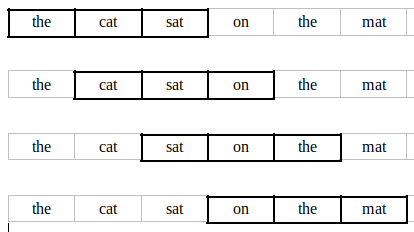
\includegraphics[width=0.75\textwidth]{diagrams/sliding-window}
  \end{center}
  \caption{Sliding Window}
  \label{fig:SlidingWindow}
\end{figure}
\FloatBarrier

The resultant tensor is typically very sparse as it counts the
frequency of all possible $n$-grams over the vocabulary $\set{V}$, and
intuitively few (if any) documents would use every possible $n$ length
combination of its vocabulary as most of these phrases would be
nonsensical.  Thus the set of tensors $\set{C}$ produced by
Algorithm~\ref{alg:BuildTensor} is a set of sparse tensors representing
the document corpus.  The last tensor in the set is the representation
of the target document as it has been placed at the end of the
document list, as mentioned previously.

\subsection{Tensor Decomposition}
The next step in the process is to decompose each document tensor into
rank 1 components.  As noted in chapter 1, several decompositions
exist which can accomplish this task.  Because the data the present
model consumes is frequency counting, the tensors comprising the
corpus are all strictly non-negative.  This arrangement naturally
lends itself to non-negative factorization.  Moreover, as these
tensors are expected to be very sparse, any factorization that admits
negative numbers would likely take a very long time to converge as it
explores many combinations of factors which sum to zero.  In fact,
these alternating negative and positive factors would necessarily
dominate the factors and would make comparison of factors very
difficult while providing no useful information about the underlying
document.  Therefore, not only is non-negative factorization a logical
choice, it is also a necessary choice to ensure the expressiveness of
the resultant model.

The method of non-negative factorization employed in this model is the
Columnwise Coordinate Descent (CCD) method described in Ji Liu et al's
paper~\cite{liu2012sparse}. The CCD method decomposes a tensor
$\tens{A}$ into a
core tensor $\tens{C}$ and a set of factor matrices $U_{1\ldots m}$
where $m$ is the number of modes.  The result of this decomposition is
shown in Equation~\ref{eq:ccd}.  The object of the model is to
minimize the error tensor $\tens{E}$, and CCD accomplishes this by
iteratively solving for $U_i$ by holding the other factor matrices
constant.  The optimal solution for each entry of $U_i$ is governed by
a differential equation which is solved iteratively (as it has no
closed form solution).  The big advantage to the CCD method is that
rows in each column are independent, and so entire columns can be
solved in parallel.  CCD also allows for $L_1$ sparsity constraints to
be applied, though this is not used in the present model.  (The $L_1$
penalty is set to 0 for this model.)  
\begin{equation}
  \label{eq:ccd}
  \tens{A} = (\tens{C} \times_1 U_1 \times_2 \ldots \times_m U_m) - \tens{E}
\end{equation}

Note that the CCD model is a non-negative version of the Tucker
decomposition. By constraining the CCD model to use a square identity
tensor (of dimension $n \times n \times \ldots n$) for
$\tens{C}$, the model becomes equivalent to the non-negative canonical
polyadic decomposition.  Each $U_i$ matrix will contain $n$ columns,
and when this product is carried out, it can be rewritten as the sum
of the tensor product of the columns of $U$.  That is, the equivalent
CP model can be written as in Equation~\ref{eq:cp-ccd}.
\begin{equation}
  \label{eq:cp-ccd}
  \tens{A} = \dsum_{i=1}^n U^1_{:,i} \otimes U^2_{:,i} \otimes \ldots
  \otimes U^m_{:,i} - \tens{E}
\end{equation}

Having extracting the rank-1 tensors which approximate $\tens{A}$, the
last remaining step is to normalize these factors.  The norm used in
this model is the $L_1$ norm.  Separating these out, the final
approximation of each document tensor is shown in
Equation~\ref{eq:cp-ccd-normalized}.
\begin{equation}
  \label{eq:cp-ccd-normalized}
  \tens{A} \approx \dsum_{i=1}^r \lambda_i \tens{F}_i
\end{equation}

The entire process of the construction of these factors is shown in
Algorithm~\ref{alg:ExtractFactors}.  The result is an $L_1$ normalized
set of rank-1 tensors.  
\begin{algorithm}
  \caption{Extract Factors}
  \label{alg:ExtractFactors}
  \SetKwData{LN}{$\set{\Lambda}$}  \SetKwData{C}{$\set{C}$}
  \SetKwData{F}{$\set{F}$} \SetKwData{U}{$\set{U}$}
  \SetKwData{T}{$\tens{T}$}\SetKwData{D}{$\tens{D}$}
  \SetKwFunction{Norm}{$\mathrm{L}_1$\_norm}
  \SetKwFunction{CCD}{ccd\_ntfd}
  \SetKwInOut{Input}{input}\SetKwInOut{Output}{output}
  \Input{\C, $nfactors$}
  \Output{\LN, \F}
  \BlankLine
  $\F \leftarrow \emptyset$\;
  $\LN \leftarrow \emptyset$\;
  $nmodes \leftarrow$ number of modes in $\C[1]$\;
  \ForEach{\D in \C}{
    $\U \leftarrow $ \CCD{\D, $nfactors$}\;
    \For{$i$ = 1 to $nfactors$}{
      \tcc{Build the Factor}
      $\T \leftarrow \U[1][:,i]$\;
      \For{$m$ = 2 to $nmodes$}{
        $\T \leftarrow \T \otimes \U[m][:,i]$\;
      }

      \tcc{Compute the norm and normalize the factor}
      $\lambda \leftarrow $\Norm{\T}\;
      $\T \leftarrow \T / \lambda$\;

      \tcc{Insert the factor and norm into the list}
      $\F \leftarrow \F \cup \{\T\}$\;
      $\LN \leftarrow \LN \cup \{\lambda\}$\;
    }
  }
  \Return{\LN, \F}
\end{algorithm}

As noted in Chapter 1, the number of factors determines the uniqueness
of the decomposition.  In the case of canonical polyadic
decomposition, the solution is unique if the number of factors exceeds
the tensor rank.  However, computing the tensor rank is intractable,
and so it must be approximated through trial and error.  One rule of
thumb for a 3-mode tensor, which is what is used in the case study in
this dissertation, is that its expected minimal rank is given in
Equation~\ref{eq:typical_rank}~\cite{comon2009}.
\begin{equation} \label{eq:typical_rank}
  R = \left\lceil \displaystyle\frac{IJK}{I+J+K-2} \right\rceil
\end{equation}
However, this estimate assumes a generic tensor and not a sparse
tensor!  In fact, in every instance of the document tensors used here,
this minimal rank would far exceed the number of non-zero elements.
This leaves the choice up to searching for a number of factors which
gives a the best fit to the model.  The approach used to find this
number begins with assuming that the non-zero elements, $nnz$, of the
document tensor were packed into a dense tensor with dimensions
$\sqrt[3]{nnz} \times \sqrt[3]{nnz} \times \sqrt[3]{nnz}$.  This
starting point is then computed using
Equation~\ref{eq:sparse_start_rank}.  From this point, decompositions
are attempted with increasing rank until the fit begins to become
worse, or until the error ratio drops below $20\%$
(Equation~\ref{eq:error_ratio}).  (Of course a different threshold
could be used if desired.)
\begin{equation}\label{eq:sparse_start_rank}
  R_0 = \left\lceil \displaystyle\frac{nnz}{3\sqrt[3]{nnz}-2} \right\rceil
  \end{equation}
  
\begin{equation}\label{eq:error_ratio}
  \displaystyle\frac{|\tens{D} - \tens{\hat{D}}|}{|\tens{D}|}
\end{equation}

\subsection{Factor Classification}
Having extracted factors from the document corpus, the next step is to
classify each of the target document's factors as either belonging to
the set $F^s_t$ (target factors with sources) or $F^n_t$ (target
factors without sources).  In order to do this, the similarity of each
factor pair must be measured.  Because each factor has the same
dimension, and each factor's modes have the same semantic meaning,
they can be compared by distance from each other within the factor
space.  Algorithm~\ref{alg:distance} accomplishes this task by finding
the $L_1$ distance between each pair of factors.  The result is a
matrix $M$ where $M_{ij}$ is the $L_1$ distance between $\set{F}_i$
and $\set{F}_j$.  Of course, this matrix will have zeroes on the
diagonal.  Because each factor is non-negative and already $L_1$
normalized, $0 \leq M_{ij} \leq 2$, where 0 is a perfect match and 2
indicates maximum distance.  
\begin{algorithm}
  \caption{Build Distance Matrix}
  \label{alg:distance}
  \SetKwData{DM}{$M$} \SetKwData{F}{$\set{F}$}
  \SetKwInOut{Input}{input}\SetKwInOut{Output}{output}
  \SetKwFunction{Norm}{$\mathrm{L}_1$\_norm}
  \Input{\F}
  \Output{\DM}
  \BlankLine
  $\DM \leftarrow $ Matrix with dimension $|\F| \times |\F|$\;
  \For{$i=1$ to $|\F|$}{
    \For{$j=1$ to $|\F|$} {
      $\DM[i,j] \leftarrow$ \Norm{$\F[i] - \F[j]$}\;
    }
  }
  \Return{\DM}
\end{algorithm}

The final task to be preformed in constructing the model is to
identify which source factors are closest to each target factor and
compute the corresponding weights of those factors.  This task is
carried out by Algorithm~\ref{alg:influence}.  The basic strategy is
for each factor in the target document to be assigned the source
factor with the minimum distance.  The only issue with this approach
is it would always assign a source to a target factor, even though
some target factors are expected to have no relatable source.  For
this reason, two steps are needed.  First, the minimum is found,
second it is compared against a threshold.  If the minimum value is
below this threshold, the factor is assigned a source.  If, on the
other hand, the minimum distance is above the threshold it is not
assigned a source.

The result of the classification operation is the set $\set{W}$ which
is simply the normalized set of $\lambda$ values for the target
document, and the set $\set{S}$ where entry $\set{S}_i$ is the index
of the factor which is the source for target factor $i$.  If target
factor $i$ has no assignable source, then a value of 0 is written to
position $\set{S}_i$.
\begin{algorithm}
  \caption{Extract Influence}
  \label{alg:influence}
  \SetKwInOut{Input}{input}\SetKwInOut{Output}{output}
  \SetKwData{DM}{$M$} \SetKwData{F}{$\set{F}$}
  \SetKwData{LN}{$\set{\lambda}$}\SetKwData{Ndocs}{$ndocs$}
  \SetKwData{W}{$\set{W}$} \SetKwData{S}{$\set{S}$}
  
  \Input{\Ndocs, \DM, \F, \LN, $threshold$}
  \Output{\W, \S}
  \BlankLine
  \tcc{Compute Weights}
  $s \leftarrow \sum \LN$\;
  $\W \leftarrow \LN / s$\;
  \BlankLine
  \tcc{Classify Factors}
  $nfactors \leftarrow |\LN|$\;
  \For{$i=1$ to $nfactors$}{
    $min \leftarrow \DM[row,1]$\;
    $minIndex \leftarrow 1$\;
    $row \leftarrow i + nfactors * (ndocs-1)$\;
    \For{$j=1$ to $nfactors * ndocs$}{
      \If{\DM[row,j]$< min$}{
        $min \leftarrow \DM[row,j]$\;
        $minIndex \leftarrow j$\;
      }
    }
    \eIf{$min \leq threshold$}{
      $\S[i]\leftarrow minIndex$\;
    }{
      $\S[i]\leftarrow 0$\;
    }
  }
  \Return{\W, \S}\;
\end{algorithm}

\section{Implementation}
Implementing the model described in this chapter comes with several
challenges.  The biggest challenge is the size of the tensors, as well
as a lack of good support for sparse tensors in available software.
Several packages were tried, but ultimately a custom tensor library
was needed to support these tensors.  The attempted software packages
were Tensor Flow (Python), Tensor Toolbox (Matlab),  SciPy/NumPy
(Python).  While all three packages provide support for sparse
tensors, their operations are not well optimized for sparse tensor
usage.  Also, in some cases, tensors were converted into dense tensors
before operations were performed.  Unconstrained vocabularies can
often have tens of thousands of words, which leads to a tensor which
far exceeds the capacity of any machines available for this project.
Before these libraries were abandoned, constrained vocabularies were
attempted.

\subsection{Constraining Vocabularies}
As already stated, the tensors used in this model are very sparse.
Essentially, every word in a document is the beginning of a new
phrase, and so every document tensor will contain the same number of
non-zero entries as there are words in the document.  (With the
exception being the last $n$-gram which is necessarily truncated.)
Storing the frequency counts of these documents is trivial, but the
model needs them in their positions within the tensor in order to
decompose and fit elements.  Most of the complexity, therefore lies
with the dimensionality of the tensor which is driven by the size of
the vocabulary.

Looking at the vocabularies in several documents during preliminary
experiments showed that each document only had about five hundred to
one thousand frequent words.  By sorting the vocabulary in descending
order by frequency, the vocabulary can be shortened with minimal
disturbance to the structure of the document and the makeup of most of
the $n$-grams.  Constraining the vocabulary to 600 words when building
a 3-gram tensor results in a tensor which has 216,000,000 potential
entries.  Even in dense format, this can be comfortably accommodated by
the memory of even a modest modern desktop machine.  However, a
problem still remains with this approach.  Decompositions of a tensor
of this size, typically into 100-200 factors, requires too much time.
Non-negative factorization tended to require about 2 hours of time,
and so a faster method was still needed even in the constrained case.
Searching for the optimal number of factors by multiple factorings
proved even more challenging.  This is especially challenging when
considering that this model requires the decomposition of multiple
documents within a corpus!

\subsection{The sptensor Library and Tool}
To address the problems of time and memory constraints, a new library
was created.  This library is called sptensor, and it is written in
ANSI C.  C was selected because it provides enough control for
optimizing memory usage and it is well situated to have libraries for
other languages bound to it.

The sptensor library is implemented as a shared library, and also has a
command line tool which allows tensor operations to be performed on
files.  The main components of the sptensor library are:
\begin{description}
\item[{\tt vector}] An array list styled general purpose storage structure.
  This grows dynamically as needed.
\item[{\tt sptensor}] A sparse tensor storage structure.  Tensors are stored
  as a list of coordinates with indexes and values stored in separate
  vectors.  The tensor indexes are maintained in sorted order giving
  $O(\mathrm{lg} n)$ lookups.
\item[{\tt tensor\_view}] A series of overlays for tensor objects.  These
  provide general ways of accessing tensors, printing tensors, and
  performing operations.  Operations included in the library are
  reshaping tensors, slicing tensors, and general tensor arithmetic.
  Mechanisms are provided to allow the library's user to provide their
  own tensor views.
\item[{\tt tensor\_math}] A set of tensor operations.  These include
  element wise operations, scalar multiplication, and a set of tensor
  products.
\item[{\tt ccd}] An implementation of Liu's Columnar Coordinate
  Descent non-negative tensor factorization algorithm~\cite{liu2012sparse}.
\end{description}

The goals for the development of this library are:
\begin{enumerate}
  \item Implement a library for dealing with sparse tensors
    efficiently.
  \item Provide fast CCD tensor decomposition.
  \item Provide an MPI implementation for common tensor functions to
    allow for operations on very large tensors.
\end{enumerate}
At the time of this writing, the first two goal have been achieved but
unfortunately the MPI version of sptensor does not yet exist.  The
sptensor library is designed to only represent sparse tensors, and so
it has the opposite problem the common tensor libraries have.  Dense
tensors are fairly inefficient both in time and space complexity.
However, for the present application the library performs quite well.
Where Matlab factorization of tensors over constrained vocabularies
typically require 1-2 hours to complete, sptensor can accomplish the
task in 5-10 minutes.  This speedup allowed for the construction and
testing of the model to proceed.

\subsection{Text Modeling Suite}
The text model described in this chapter is implemented as a series of
stand-alone programs.  Essentially, each of the above algorithms are
implemented as either part of the sptensor library or as a stand alone
utility.  The decision of whether to build an algorithm into sptensor
was based on whether the operation was a generic tensor operation, or
whether it was specific to this model.  The sptensor tool provides the
following facilities:
\begin{itemize}
\item CCD Factorization (as used in
  Algorithm~\ref{alg:ExtractFactors}.
\item Extraction of normalized factors from the matrix output of CCD,
  also from Algorithm~\ref{alg:ExtractFactors}.
\item Distance matrix computation (Algorithm~\ref{alg:distance})
\end{itemize}

In addition to the sptensor utility, the following stand alone
programs are used to build the model:
\begin{description}
\item[prepare] This is a simple bash shell script which uses the UNIX
  command tr to perform the filtering and lower case conversion found
  in Algorithm~\ref{alg:distance}.
\item[vocabulary] A small python program that reads all the documents
  in a corpus, builds a vocabulary, and counts word frequencies.  The
  vocabulary is then sorted and truncated to a desired length.  An @
  symbol is inserted at the end as a wildcard for all the infrequent
  words.  The output of this program is a vocabulary file, which
  simply lists each word in the vocabulary one per line.
\item[doctns] A C program which uses the sptensor library to build the
  document tensors according to Algorithm~\ref{alg:BuildTensor}.  If
  doctns encounters a word not in the vocabulary, it uses the wildcard
  at the end of the list.
\item[classify] A C program which uses the sptensor library to
  classify and report classification of factors.  The output of this
  corresponds to the$\set{S}$ and $\set{W}$ sets in Algorithm~\ref{alg:model}.
\item[build-model] A shell script which invokes all the other
  programs as per Algorithm~\ref{alg:model}.
\end{description}

\end{document}
